\subsubsection{Data Augmentation?}
\paragraph{}
As we mentioned before we face a problem of imblanced data set while using fer2013 dataset ,so we check this technique as an over sampling method.and we will give a breif about it.
\paragraph{what is Data Augmentation?}
Data augmentation is a technique to artificially create new training data from existing training data. This is done by applying domain-specific techniques to examples from the training data that create new and different training examples.
\paragraph{}
Image data augmentation is perhaps the most well-known type of data augmentation and involves creating transformed versions of images in the training dataset that belong to the same class as the original image.
\paragraph{}
Transforms include a range of operations from the field of image manipulation, such as shifts, flips, zooms, and much more.
\paragraph{}
The intent is to expand the training dataset with new, plausible examples. This means, variations of the training set images that are likely to be seen by the model. For example, a horizontal flip of a picture of a cat may make sense, because the photo could have been taken from the left or right. A vertical flip of the photo of a cat does not make sense and would probably not be appropriate given that the model is very unlikely to see a photo of an upside down cat.
\paragraph{}
As such, it is clear that the choice of the specific data augmentation techniques used for a training dataset must be chosen carefully and within the context of the training dataset and knowledge of the problem domain. In addition, it can be useful to experiment with data augmentation methods in isolation and in concert to see if they result in a measurable improvement to model performance, perhaps with a small prototype dataset, model, and training run.
\paragraph{}
Modern deep learning algorithms, such as the convolutional neural network, or CNN, can learn features that are invariant to their location in the image. Nevertheless, augmentation can further aid in this transform invariant approach to learning and can aid the model in learning features that are also invariant to transforms such as left-to-right to top-to-bottom ordering, light levels in photographs, and more.
\paragraph{}
Image data augmentation is typically only applied to the training dataset, and not to the validation or test dataset. This is different from data preparation such as image resizing and pixel scaling; they must be performed consistently across all datasets that interact with the model.
\begin{figure}
	\centering
	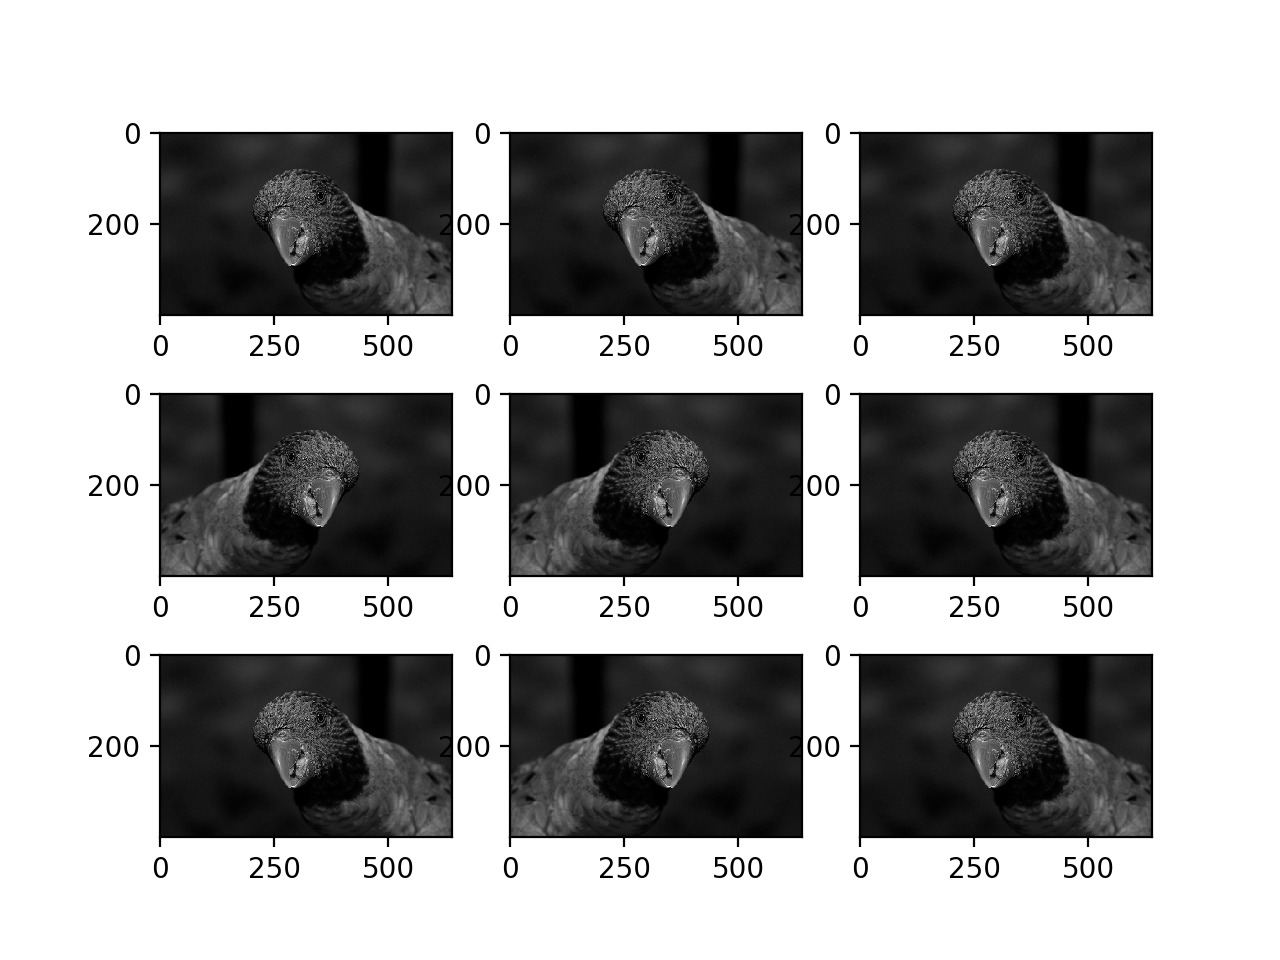
\includegraphics[width=1\textwidth]{data_aug.jpg}
	\caption{example of Data Augmentation "Horizontal flip"}
\end{figure} 
\subsubsection{Results}

